Para realizar o desenvolvimento do circuito, foi utilizado o simulador \textit{Falstad} (disponível em: \href{https://www.falstad.com/circuit/circuitjs.html}{falstad.com/circuit/circuitjs.html}). Como pode ser observado na Figura ~\ref{fig:circuit_svg}, foi simulado um circuito para a conversão de sinais de $1\, \text{Hz}$ de entrada alternada, com $5\, \text{Vpp}$.


\begin{figure}[H]
    \centering
    \resizebox{1\linewidth}{!}{%
        \includesvg{03_results/assets/circuit-20241128-2341.svg}
    }
    \caption{Diagrama do circuito de conversor analógico-digital Rampa Dupla}
    \label{fig:circuit_svg}
\end{figure}

Na etapa de construção do circuito, foram utilizados um resistor de $10\, \text{k} \Omega$ e um capacitor de $1\, \text{nF}$ no estágio integrador do conversor.

No desenvolvimento do conversor analógico-digital por Rampa Dupla, um aspecto essencial a considerar é a relação entre a frequência do sinal de entrada, a quantidade de níveis de quantização e o clock utilizado no contador. Para este projeto, determinamos inicialmente a quantidade de amostras que queremos ter em um período do sinal. Definimos esse valor em 250, ou seja, a cada 1/250 períodos da onda, o circuito realizará um ciclo completo de integração e desintegração. Com esse valor obtêm-se uma boa resolução sem um clock muito alto. Como nossa entrada é de $1\, \text{Hz}$, esse período é $1\,\text{s}$, então a cada $4\, \text{ms}$, teremos as duas rampas. O período de integração é de metade do período máximo de amostragem, $T_{1} = 2\, \text{ms}$.

Podemos verificar que um período de integração de $2\, \text{ms}$ resulta em um $T_{max} = 4\, \text{ms}$ utilizando a relação a seguir:

\begin{align*}
    T_{\text{max}}  & = T1 + T_{2\text{max}}                                          \\
    T_{2\text{max}} & = T1                                                            \\
    T_{\text{max}}  & = 2^{N} \times T_{\text{clock}} + 2^{N} \times T_{\text{clock}} \\
    T_{\text{max}}  & = 2 \times 2^{N} \times T_{\text{clock}}                        \\
    T_{\text{max}}  & = 2^{6+1} \times 0.00003125                                     \\
    T_{\text{max}}  & = 4 \text{ ms}
\end{align*}


A partir dessas definições, definimos o clock que será utilizado no contador para a obtenção do tempo de integração desejado de $2\, \text{ms}$:

\begin{align} \
    T_{1} = \frac{2^N}{f_{clock}} \\
    T_{1} = 2^N \cdot T_{clock}
\end{align}

onde:
\begin{enumerate}
    \item $T_1$ é o tempo total de integração ($2\, \text{ms}$)
    \item $2^N$ é o número de níveis de quantização (relacionado ao número de bits do conversor, $N$),
    \item $T_{clock}$ é o período do sinal de clock.
\end{enumerate}

Rearranjando a fórmula para encontrar $T_{clock}$, temos:

\begin{align} \
    T_{clock} = \frac{T_{1}}{2^N}               \\
    \text{Adotando} \, N=6 \, \text{bits:} \,
    T_{clock} = \frac{2 \times 10^{-3}}{64}     \\
    T_{clock} = 31.25 \times 10^{-6}\, \text{s} \\
    T_{clock} = 31.25\, \mu\text{s}
\end{align}

Assim, a frequência do clock ($f_{clock}$) é o inverso do período:

\begin{align} \
    f_{clock} = \frac{1}{T_{clock}}            \\
    f_{clock} = \frac{1}{31.25 \times 10^{-6}} \\
    \therefore f_{clock} \approx 32\, \text{kHz}
\end{align}

Portanto, o circuito deve operar com uma frequência de clock de $32\, \text{kHz}$ para realizar o processo de conversão com $2\, \text{ms}$ de período de integração.


Assim temos uma quantidade mínima de $\frac{1\, \text{s}}{0.004\text{s}(2ms*2)\ }$ amostras por período do sinal de entrada, ou seja 250 amostras por período.

A partir da Figura ~\ref{fig:falstad_simulator_output}, é possível observar duas representações gráficas dos sinais envolvidos no funcionamento do conversor analógico-digital (ADC) de Rampa Dupla. Na imagem B, está representada a entrada analógica alternada, um sinal senoidal de $1\, \text{Hz}$ com amplitude de $5\, \text{Vpp}$, que é o dado a ser convertido. Já na imagem A, temos a saída do circuito integrador, e a saída digital correspondente, que apresenta o sinal já amostrado e quantizado pelo ADC.

\begin{figure}[H]
    \centering
    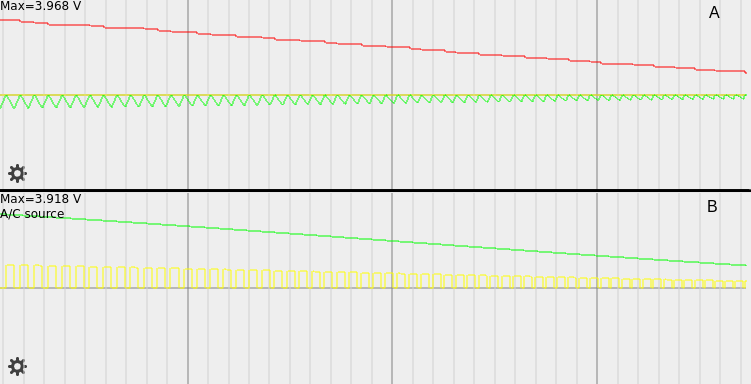
\includegraphics[width=1\linewidth]{03_results/assets/signal_output.png}
    \caption{A: Saída do ADC; B: Entrada A/C}
    \label{fig:falstad_simulator_output}
\end{figure}

O sinal quantizado e digitalizado, exibido na imagem A, reflete a discretização imposta pelo ADC. Cada degrau no gráfico representa um dos 64 níveis disponíveis no intervalo de operação, evidenciando o mapeamento do sinal senoidal contínuo em valores digitais. Nota-se que a resolução de 6 bits implica que a precisão do ADC depende tanto da estabilidade do clock quanto da qualidade do circuito integrador.

\subsection{Reduzindo para 25 amostras por período}
Caso a quantidade de amostras seja reduzida de 250 para 25 amostras por período do sinal de entrada, o período de amostragem aumenta proporcionalmente, passando de $4\,\text{ms}$ para $40\, \text{ms}$. Consequentemente, o tempo de integração ($T_1$) será de $20\, \text{ms}$, conforme definido anteriormente como metade do período de amostragem. A partir disso, podemos calcular a frequência de clock necessária.

Usando a mesma fórmula básica e adotando $N=6\,\text{bits}$, temos:
$$
    f_{clock} = \frac{2^N}{T_{1}} = \frac{64}{20 \times 10^{-3}} = 3.2 \, \text{kHz}
$$

Assim, ao reduzir a quantidade de amostras para 25, a frequência do clock também diminui para \textbf{$3.2 \, \text{kHz}$}. Essa alteração resulta em um menor consumo de energia e em um design menos exigente em termos de velocidade, ao custo de uma resolução temporal menor para o sinal de entrada.

Na Figura ~\ref{fig:falstad_simulator_output_25_samples}, observamos a saída do circuito operando com 25 amostras por período. Os principais pontos de inflexão do sinal ainda são capturados, mas há uma perda de detalhes na representação digital devido à menor densidade de amostras.

\begin{figure}[H]
    \centering
    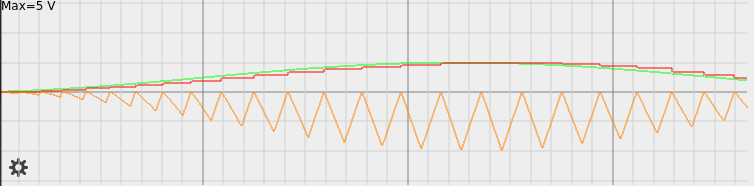
\includegraphics[width=1\linewidth]{03_results/assets/signal_output_25_samplings.png}
    \caption{Entrada A/C(verde), Saída Integrador (laranja), Saída Digital (vermelho)}
    \label{fig:falstad_simulator_output_25_samples}
\end{figure}

A perda de detalhes se dá devido à menor capacidade do ADC de acompanhar as rápidas variações do sinal de entrada. Em caso de sinais mais complexos ou de maior frequência, pode haver a introdução de maiores erros na representação digital do sinal.
